\graphicspath{{chapters/loadings/}}


\chapter{Insights From Generating Simulated Data for CCA: Loadings not Weights}\label{chap:loadings}
\epigraph{Correlation does not imply causation.}{\textit{Anon.}}
\minitoc
% chktex-file 44
% chktex-file 3
\section*{Preface}

This chapter, deriving insights from various projects, primarily unpublished, delves into the application of loadings over weights for model interpretation in CCA models. The simulated data generation methods were used to generate simulated data in \citet{mihalik2022canonical}. The arguments for the use of loadings influenced our choice of loadings for the interpretation of the results in \citet{}.

\section{Introduction}

There remains a substantial debate in the \acrshort{cca} literature about the relative merits of interpreting models in terms of weights or loadings \citep{gu2018simultaneous}.
Simulated data has also been used extensively to understand the properties of \acrshort{cca} models for high-dimensional data \citep{chen2013sparse, suo2017sparse, helmer2020stability} including the recovery of sparse weights.

In this chapter, we first review the generative perspectives on \acrshort{cca} and show that they can be categorized into two groups: explicit latent variable models and implicit latent variable models, in particular by reformulating the joint covariance matrix perspective used by \citet{suo2017sparse, chen2013sparse, helmer2020stability} as an implicit latent variable model.

This rigorous categorization of generative approaches to \acrshort{cca} is novel and gives both a unique perspective on both the merits of weights and loadings, and understanding the properties of \acrshort{cca} models in high-dimensional simulations.
We also make a mathematical argument for the use of loadings over weights for the interpretation of \acrshort{cca} models, showing that the \gls{loadings} are invariant to columnwise transformations of the data matrix, while the weights are not.

We illustrate these arguments with simulated data and revisit the results from chapter \ref{chap:als} through the lens of loadings.

\section{Background}

In practical applications, (\acrshort{cca}) has two aspects: estimating latent variables associated with different views, and exploring the expression of these latent variables in each view, ideally providing insight into biomedical mechanisms.
These aspects correspond to the motivation behind discriminative and generative approaches in machine learning.

\paragraph{Generative} approaches in CCA seek to understand the data generation process.
They are concerned with the joint distribution $P(X\sps{1},X\sps{2})$ and the conditional distribution $P(X\sps{1},X\sps{2}|Z)$.
We will refer to this conditional distribution as the `forward model', since it describes how the observed data are generated from the latent variables.
This model is parameterized by `loadings' which describe the relationship between the latent variables and the observed data.
\paragraph{Discriminative} approaches in \acrshort{cca} prioritize estimating latent variables from observed data, typically employing `weights' as parameters.
In the context of the graphical model of \acrshort{cca} in Figure~\ref{fig:forward-backward-models}, discriminative approaches estimate the distribution $P(Z|X\sps{1},X\sps{2})$.
We will refer to this conditional distribution as the `backward model', since it describes how we can infer the latent variables from the observed data.

\begin{figure}
    \centering
    \tikz{
    % nodes
        \node[latent, align=center, minimum size=2cm] (Z) {Severity\\z};
        %
        \node[obs, below left=of Z, minimum size=2cm, align=center] (x1) {Brain\\$x^{(1)}$};
        \node[obs, below right=of Z, minimum size=2cm, align=center] (x2) {Behaviour\\$x^{(2)}$};
        % edges
        \edge[blue]{Z} {x1};
        \edge[blue]{Z} {x2};
        \edge[red, tension=0.1]{x1} {Z};
        \edge[red, tension=0.1]{x2} {Z};
    }
    \caption[Forward and Backward Multiview Models]{\textit{\textbf{Forward and Backward Multiview Models:}} The \textcolor{blue}{generative approach to \acrshort{cca} focuses on the forward model from latent variables to observed data}, while the \textcolor{red}{machine learning approach focuses on the backward model from observed data to latent variables}.}\label{fig:forward-backward-models}
\end{figure}

\citet{gu2018simultaneous} noted that there appear to be two schools of thought in the \acrshort{cca} literature: one that focuses on the weights and one that focuses on the loadings.
The former group argues both that the weights provide a measure of the contribution of each feature holding other features constant, and that weights are multivariate.
The latter group argues that the loadings are more interpretable because they measure how much each feature is represented by the latent variable.
\citet{haufe2014interpretation} argued for the use of loadings for interpretability in the context of linear models like SVM and Lasso in neuroimaging.
\citet{alpert1972interpretation} also highlighted the problem with interpreting weights in the backward model, noting that they inherit all of the problems of interpreting regression coefficients.
They conclude that weights appear more suitable for prediction, while correlations may better explain underlying (although interrelated) constructs.

In this chapter, we are interested in generating insights to the interpretability of \acrshort{cca} models in the context of simulated data where we know precisely how the data were generated.
The most important argument we will make is that all generative approaches to \acrshort{cca} are implicitly latent variable models, so that loadings are the natural parameters for interpretation.

\section{Unifying Generative Perspectives on \acrshort{cca}}\label{sec:generative-perspectives}

In this section, we review the generative perspectives on \acrshort{cca} and show that they can be categorized into two groups: explicit latent variable models and implicit latent variable models.

\subsection{Probabilistic \acrshort{cca} and \acrshort{gfa} (Explicit Latent Variable Models)}

Let's reconsider the graphical model depicted in Figure~\ref{fig:forward-backward-models}.
Now we further assume that the brain is generated via a linear model with added noise, while the behavioural modality similarly arises from a linear model with noise.
Once again they are conditionally independent, given the latent variable.

The distributions of the two views are given by:

\begin{align}
    z& \sim \mathcal{N}(0, I)\\
    x\sps{i} & \sim \mathcal{N}(W\sps{i} z + \mu\sps{i}, \Psi\sps{i})
\end{align}

Where \(z\) represents the latent variable (disease severity), \(x\sps{i}\) represents the $i^{\text{th}}$ view, \(W\sps{i}\) represents the model loadings, \(\mu\sps{i}\) represents the mean, and \(\Psi\sps{i}\) represents the noise covariance matrix for the $i^{\text{th}}$ view.
Notice that if it were not for the view-specific noise, the two views would be perfectly correlated subject to a linear transformation.

\citet{bach2005probabilistic} showed that the maximum likelihood solution for this model is equivalent to the solution of the \acrshort{cca} problem in the sense that the \gls{loadings} are the same as the \acrshort{cca} weights multiplied by the covariance:

\begin{align}
    \label{eq:probabilistic-cca}
    \hat{W}\sps{i} = \Sigma_{ii} \hat{U}\sps{i} R
\end{align}

Where $R$ is an arbitrary rotation matrix and $\hat{U}\sps{i}$ is the matrix of \acrshort{cca} weights for the $i$th view.
This implies that for invertible covariance matrices, we can access the `true' \acrshort{cca} weights associated with the top-k subspace by multiplying the \gls{loadings} by the inverse of the covariance matrix:

\begin{align}
    \hat{U}\sps{i}R = \Sigma_{ii}^{-1} \hat{W}\sps{i}
\end{align}

In practice we do not have access to the covariance matrices $\Sigma_{ii}$, so we must estimate them from the data using the sample covariance matrices $\hat{\Sigma}_{ii}$.

\textbf{Notice that for Identity covariance matrices, the \acrshort{cca} weights are the same as the loadings.}
Otherwise, there is a linear transformation between the two.
For singular covariance matrices, the \acrshort{cca} weights are not uniquely defined.

Moreover, the mean of the posterior distribution of the latent variables is proportional to the mean of the \acrshort{cca} scores \citep{klami2013bayesian}.
Group Factor Analysis (\acrshort{gfa}) is a closely related model that assumes diagonal covariance in $\Psi\sps{i}$:

\begin{align}
    z& \sim \mathcal{N}(0, I)\\
    x\sps{i} & \sim \mathcal{N}(W\sps{i} z, \sigma\sps{i}I)
\end{align}

An interesting feature of the \acrshort{gfa} model is that as the noise level approaches zero, the marginal distribution of the views is the same as the probabilistic PCA model for each view~\citep{tipping1999probabilistic}.
This suggests that for small noise levels, we should in fact be able to recover much of the mutual information between the views by using PCA on each view separately.
For this reason, we will use and recommend PCA as a baseline in our later experiments.
Because the diagonal covariance assumption makes inference computationally cheaper, this line of work has been able to extend to incorporate sparsity on the loadings~\citep{virtanen2011bayesian} as well as missing data~\citep{ferreira2022hierarchical}.

By marginalizing out the latent variables of the generative \acrshort{cca} and \acrshort{gfa} models, we can write down the joint distribution of the two views:

\begin{align}
    \begin{bmatrix}
        X\sps{1} \\ X\sps{2}
    \end{bmatrix} \sim \mathcal{N} \left( \begin{bmatrix}
                                              \mu\sps{1} \\ \mu\sps{2}
    \end{bmatrix}, \begin{bmatrix}
                       W\sps{1}W\spsT{1} + \Psi_1 & W\sps{1}W\spsT{2} \\ W\sps{2}W\spsT{1} & W\sps{2}W\spsT{2} + \Psi_2
    \end{bmatrix} \right)
\end{align}

Importantly, this shows us that the true covariance in each view is a function of the \gls{loadings} and the noise covariance matrix.
Specifically, the covariance matrix of the $i^{\text{th}}$ view is given by:

\begin{align}
    \Sigma_{ii} = W\sps{i}W\spsT{i} + \Psi_i
\end{align}

While these generative models are provide a clear interpretation of the data generation process and possible biological processes, their application in practice is limited compared to classical \acrshort{cca}.
This is primarily due to their computational intensity and the need for a careful selection of priors.
Moreover, while these models can generate data with sparse loadings, generating data with sparse weights is challenging due to the dependence of \acrshort{cca} weights on the covariance matrices of the views.

\subsection{Joint Covariance Matrix Perspective (Implicit Latent Variable Model)}

In contrast to the explicit latent variable models discussed earlier, the joint covariance matrix perspective \cite{suo2017sparse,chen2013sparse} offers an implicit approach to understanding the data generation process.
This method focuses on the covariance matrices of the views, rather than directly modeling latent variables.
A key advantage of this perspective, particularly noted in the sparse \acrshort{cca} literature, is its ability to generate data with known sparse weights and or known canonical correlations.
This is achieved by constructing the joint covariance matrix of the distribution $P(X\sps{1},X\sps{2})$:

\begin{align}
    \label{eq:covariance}
    \begin{bmatrix}
        X\sps{1} \\ X\sps{2}
    \end{bmatrix} \sim \mathcal{N} \left( \begin{bmatrix}
                                              0 \\ 0
    \end{bmatrix}, \begin{bmatrix}
                       \Sigma_{11} & \Sigma_{12} \\ \Sigma_{21} & \Sigma_{22}
    \end{bmatrix} \right)
\end{align}

Where $\Sigma_{11}$ and $\Sigma_{22}$ are the within-view covariance matrices and $\Sigma_{12}$ and $\Sigma_{21}$ are the between-view covariance matrices.

This has the advantage of allowing us to control the within-view covariance and therefore test the methods under specific conditions.
The process was first described by Chen~\citep{chen2013sparse} and further explained by~\citep{suo2017sparse} and has been the basis behind findings in \citet{helmer2020stability,matkovivc2023static}.

We can control the true signal by setting the active variables and correlations in the between-view covariance matrices $\Sigma_{12}$ and $\Sigma_{21}$.
Specifically we construct the between-view covariance matrices as follows:

\begin{align}
    \Sigma_{12}=\sum_{k=1}^{K}\rho_k\Sigma_{11}u\sps{1}_{k}u\spsT{2}_k\Sigma_{22}
\end{align}

Where $\rho_k$ is the $k^{\text{th}}$ canonical correlation and $u\sps{i}_k$ is the $k^{\text{th}}$ column of the matrix of weights $U\sps{i}$.

We can still access the true \gls{loadings} of the implied latent variable model by using the relationship in~\ref{eq:probabilistic-cca} and multiplying the weights $u\sps{i}$ by the within-view covariance matrix $\Sigma_{ii}$.

\subsection{Summary of Data Generation Methods}

\paragraph{Comparison of Joint Covariance Matrices}
To understand the distinct approaches of each data generation method, we present a comparison of their covariance structures.
This comparison highlights the differences in how these methods model the relationship within and between views.
            {
    \renewcommand{\arraystretch}{2.5} % Increase the row height
    \begin{table}[h]
        \centering
        \caption{Covariance Structures in Data Generation Methods}
        \begin{tabular}{|c|c|c|c|}
            \hline
            \textbf{}                                           & \textbf{Method}              & \textbf{Within-view Covariance} $\boldsymbol{\Sigma_{ii}}$ & \textbf{Between-view Covariance} $\boldsymbol{\Sigma_{12}}$ \\
            \hline
            \multirow{2}{*}{\rotatebox[origin=c]{90}{Explicit}} & Probabilistic \acrshort{cca} & $W^{(i)}W^{(i)\top} + \Psi_i$ & $W\sps{1}W^{(2)\top}$ \\
            \cline{2-4}
            & \acrshort{gfa}               & $W\sps{1}W^{(1)\top} + \sigma\sps{1} I$                    & $W\sps{1}W^{(2)\top}$                                                 \\
            \hline
            \multirow{2}{*}{\rotatebox[origin=c]{90}{Implicit}} & Joint Covariance             & $\Sigma_{ii}$ & $\sum_{k=1}^{K}\rho_k\Sigma_{11}u\sps{1}_{k}u^{(2)\top}_k\Sigma_{22}$ \\
            \cline{2-4}
            & Joint Covariance (Identity)  & $I$                                                        & $\sum_{k=1}^{K}\rho_ku\sps{1}_{k}u^{(2)\top}_k$                       \\
            \hline
        \end{tabular}
        \label{table:covariance-structures}
    \end{table}
}

\paragraph{Comparison of True Weights and Loadings}
We summarize the relationship between the weights and \gls{loadings} in each data generation method, distinguishing between population and sample cases.
This distinction is crucial, especially in scenarios where the population covariance matrix \( \Sigma \) is identity, but the sample covariance matrix \( \hat{\Sigma} \) is only an approximation.

\begin{table}[h]
    \centering
    \caption{Relationship Between Weights and Loadings in Population and Sample Cases}
    \begin{tabular}{|c|c|c|c|c|}
        \hline
        \textbf{}                                           & \textbf{Method}                 & \textbf{Case} & \textbf{Weights}                            & \textbf{Loadings}                \\
        \hline
        \multirow{4}{*}{\rotatebox[origin=c]{90}{Explicit}} & Probabilistic \acrshort{cca} & Population & $(W^{(i)}W^{(i)\top} + \Psi_i)^{-1}W^{(i)}$ & $W^{(i)}$ \\
        &                                 & Sample        & $\hat{\Sigma_{ii}}^{-1}W^{(i)}$             & $W^{(i)}$                        \\
        \cline{2-5}
        & \acrshort{gfa}                  & Population    & $(W^{(i)}W^{(i)\top} + I)^{-1}W^{(i)}$      & $W^{(i)}$                        \\
        &                                 & Sample        & $\hat{\Sigma_{ii}}^{-1}W^{(i)}$             & $W^{(i)}$                        \\
        \hline
        \multirow{4}{*}{\rotatebox[origin=c]{90}{Implicit}} & Joint Covariance (Non-Identity) & Population & $U^{(i)}$ & $\Sigma_{ii}U^{(i)}$ \\
        &                                 & Sample        & $U^{(i)}$                                   & $\hat{\Sigma_{ii}}\hat{U^{(i)}}$ \\
        \cline{2-5}
        & Joint Covariance (Identity)     & Population    & $U^{(i)}$                                   & $U^{(i)}$                        \\
        &                                 & Sample        & $U^{(i)}$                                   & $\hat{\Sigma_{ii}}\hat{U^{(i)}}$ \\
        \hline
    \end{tabular}
    \label{tab:weights-loadings-population-sample}
\end{table}

\subsection{Efficient Sampling of Simulated CCA Data}

Efficient sampling from high-dimensional multivariate normal distributions is a critical step in simulating data for Canonical Correlation Analysis (CCA). Traditional methods can be computationally intensive and storage-demanding, especially for large datasets. To address these challenges, we leverage low-rank and sparse covariance matrices, along with Singular Value Decomposition (SVD), to facilitate efficient and feasible sampling procedures.

\subsubsection{Challenges with High-Dimensional Data}
In the context of high-dimensional data, direct sampling from a multivariate normal distribution and storing the full covariance matrix (\(p \times p\) for \(p\) dimensions) become impractical.
High computational cost and substantial storage requirements necessitate more efficient approaches.

\subsubsection{Utilizing Low-Rank Covariance Matrices}
A practical solution is to use low-rank approximations of covariance matrices. Instead of storing the entire covariance matrix, we store only the significant components, specifically the matrices \(U\) and \(S\) from the SVD of the covariance matrix (\(\Sigma = U S U^T\)). Sampling then involves generating samples from a standard univariate normal distribution and transforming them using these SVD components.

\subsubsection{Sparse Covariance Matrices}
For certain applications, sparse covariance matrices offer an additional avenue for efficiency.
These matrices, with many zero entries, reduce both computational complexity and storage requirements, allowing for faster processing and less memory usage.

\subsubsection{Explicit Latent Variable Models}
In explicit latent variable models, we generate orthogonal latent variables from a low-dimensional multivariate normal distribution.
These are then transformed using the loading matrices to create the signal component of the data. Noise is added by sampling from a univariate normal distribution and multiplying by a factorized (low-rank or sparse) covariance matrix.
This method allows for precise control over the signal-to-noise ratio in the simulated data.

\subsubsection{Implicit Latent Variable Models}
Implicit latent variable models pose a greater challenge as they typically require storing the full covariance matrix.
However, we can improve the efficiency by employing the SVD of the covariance matrix.
This approach involves decomposing the covariance matrix and then using the resulting components to transform samples from a standard multivariate normal distribution, thereby generating samples that conform to the desired high-dimensional distribution with reduced computational overhead.

These methods collectively enhance the feasibility and efficiency of simulating CCA data, especially in high-dimensional scenarios, providing a robust framework for research and analysis in various fields.

\section{A Mathematical Argument for Using Loadings not Weights for Interpretation of CCA Models}\label{sec:an-argument-for-the-use-of-loadings}

In this section, we make a mathematical argument for the use of \gls{loadings} over weights for the interpretation of \acrshort{cca} models.
In particular, we show that the \gls{loadings} are invariant to columnwise transformations of the data matrix, while the weights are not.

\acrshort{cca} can be solved in the principal component space. Consider the singular value decomposition (SVD) of the data matrices:

\begin{align}
    X\sps{i} = U\sps{i}\Sigma\sps{i}V^{i\top} \label{eq:svd}
\end{align}

Here, $U\sps{i}$ and $V\sps{i}$ are the left and right singular vectors of $X\sps{i}$ respectively, and $\Sigma\sps{i}$ is a diagonal matrix of singular values.
The intuition behind this decomposition is that we are representing the data matrix in terms of its fundamental components: the directions of maximum variance (captured by $V\sps{i}$), the scale of these directions (captured by $\Sigma\sps{i}$), and the projections of the data onto these directions (captured by $U\sps{i}$).
$U\sps{i}$ are the principal components of $X\sps{i}$.

Substituting Equation \ref{eq:svd} into the \acrshort{cca} objective function, we have:

\begin{align}
    \max_{U\sps{1}, u\sps{2}} \Corr(X\sps{1}U\sps{1}, X\sps{2}u\sps{2}) &= \max_{U\sps{1}, u\sps{2}} \Corr(U\sps{1}\Sigma\sps{1}V^{1\top}U\sps{1}, U\sps{2}\Sigma\sps{2}V^{2\top}u\sps{2}) \label{eq:cca_obj}
\end{align}

Reparameterizing the weights as $v\sps{i} = \Sigma\sps{i}V^{i\top}u\sps{i}$, we obtain:

\begin{align}
    \max_{v\sps{1}, v\sps{2}} \Corr(U\sps{1}v\sps{1}, U\sps{2}v\sps{2}) \label{eq:reparam}
\end{align}

This reparameterization simplifies the optimization problem in two ways.
Firstly, if the data matrices are low rank (which is guarenteed if the number of samples is less than the number of features), then the matrix of principal components $U\sps{i}$ is lower dimensional than the data matrix $X\sps{i}$, reducing the number of parameters in the optimization problem.
Secondly, the reparameterization ensures that $v\spsT{1}U\spsT{1}U\sps{1}v\sps{1}=v\spsT{1}v\sps{1}$, making the constraints independent of the data.
We can therefore solve the CCA problem by solving the simpler PLS problem in the principal component space.
, which is computationally more feasible but also gives us a convenient way to understand how the weights and \gls{loadings} of \acrshort{cca} models change under different transformations of the data.

\textbf{Definition:} \textit{Loadings} are defined using the reparameterized weights as follows:

\begin{align}
    w\sps{i}_j = \Corr(X\sps{i}_j, U\sps{i}v\sps{i}) = \frac{\Cov(X\sps{i}_j, U\sps{i}v\sps{i})}{\sqrt{\Var(X\sps{i}_j)}\sqrt{\Var(U\sps{i}v\sps{i})}} \label{eq:loading_def}
\end{align}

By convention, and without loss of generality, we standardize the latent variables to have unit variance so that:

\begin{align}
    w\sps{i}_j = \frac{\Cov(X\sps{i}_j, U\sps{i}v\sps{i})}{\sqrt{\Var(X\sps{i}_j)}} \label{eq:standardized_loading}
\end{align}

Intuitively, \gls{loadings} measure how much each original feature contributes to the latent variables, providing insight into the structure of the data.

\subsection{Invariance to Scale}\label{subsubsec:invariance-to-scale}

First, we show that the \gls{loadings} are invariant to column-wise scaling of the data matrix whereas the weights are not.

\begin{lemma}
    Scaling the columns of the data matrix does not affect the left singular vectors $U\sps{i}$.
\end{lemma}

\begin{proof}
    Scale the columns of the data with a matrix \( C \):

% LaTeX equation showing C as a diagonal matrix
    \begin{equation}
        C = \begin{pmatrix}
                c_{11} & 0      & \cdots & 0      \\
                0      & c_{22} & \cdots & 0      \\
                \vdots & \vdots & \ddots & \vdots \\
                0      & 0      & \cdots & c_{nn}
        \end{pmatrix}
    \end{equation}

    where \( c_{ii} \) represents the scaling factor for the \( i \)-th column of the data matrix. For columns that are not scaled, \( c_{ii} = 1 \).
    This means that the corresponding column remains unchanged.

    Since $C$ is diagonal it can be represented by a diagonal matrix $S=C$ and an orthogonal matrix (the identity matrix) $R$.
    The transformed dataset is therefore \( X^{(1')} = X^{(1)}C \):

    \begin{align}
        X\sps{1'} = U\sps{i}\Sigma\sps{i}V^{i\top}C = U\sps{i}(\Sigma\sps{i} S\sps{i}) (\sps{i}V^{i\top}I) =  \label{eq:scaled_data}
    \end{align}

    which makes clear that the left and right singular vectors \( U\sps{i} \) and \( V\sps{i} \) right remain unchanged.
    Therefore, the modified equation can be represented as:
    \begin{equation}
        X\sps{1'} = U^i \Sigma\sps{i'} (V\sps{i})^T \label{eq:modified_svd}
    \end{equation}

    where $\Sigma\sps{i'}=\Sigma\sps{i} S\sps{i}$.
\end{proof}

\paragraph{Intuition}
Scaling the data is like changing the units of measurement.
It stretches or compresses the data but does not change the relationships between the samples.

Noting that the CCA optimisation problem remains the same as in Equation \ref{eq:reparam},
we can now show that the weights are not invariant to scaling of the data matrix but the \gls{loadings} are.

\paragraph{Weights change}

From the earlier reparameterization, and given that $v\sps{i'}=v\sps{i}$, the weights post-scaling are:

\begin{align}
    u\sps{i'} = V\sps{i}(\Sigma\sps{i'})^{-1}v\sps{i} = V\sps{i}(\Sigma\sps{i'})^{-1}v\sps{i} = C^{{(i)}^{-1}}u\sps{i} \label{eq:weights_change}
\end{align}

which are the original weights scaled by the inverse of the scaling matrix \( C \). This means that the weights are not invariant to scaling of the data matrix. Furthermore it means we can set the weights to arbitrary values by scaling the data matrix.
While we can build pipelines with standardized data, there is no a priori reason to do so.

\paragraph{Loadings are invariant}

Since \gls{loadings} are correlations between the original features and the latent variables, they are invariant to scaling of the data.
This follows from the definition of correlation and the unchanged latent variables:

\begin{align}
    w\sps{i}_j = \Corr(X\sps{i'}_j, U\sps{i}v\sps{i}) = \Corr(c_{jj}X\sps{i}_j, U\sps{i}v\sps{i}) = \Corr(X\sps{i}_j, U\sps{i}v\sps{i}) \label{eq:loading_invariant}
\end{align}

\paragraph{Intuition}
The \gls{loadings} remain the same because scaling the data does not change the relative contributions of each feature to the latent variables.

\subsection{Invariance to Repeated Linear Combinations of Columns}\label{subsubsec:invariance-to-linear-combinations}

We can also prove a more general result that the \gls{loadings} are invariant to repeated linear combinations of columns of the data matrix.
This is not as contrived as it sounds, since we often need to decide which features to include or exclude in a model, and when we work with highly correlated variables like survey questions, we may choose to use summary scores instead of individual questions.

\begin{lemma}
    Adding linear combinations of columns to the data matrix does not affect the left singular vectors $U\sps{i}$.
\end{lemma}

\begin{proof}
    Now, consider adding columns that are linear combinations of existing columns in \( X\sps{i} \) to form \( X\sps{i''} \).
    We can represent this using a transformation matrix \( A \) such that \( X\sps{i''} = X\sps{i}A \):

%A is an identity matrix horizontally concatenated with another random matrix
    \begin{equation}
        A = \begin{pmatrix}
                1      & 0      & \cdots & 0      & a_{11} & a_{12} & \cdots & a_{1m} \\
                0      & 1      & \cdots & 0      & a_{21} & a_{22} & \cdots & a_{2m} \\
                \vdots & \vdots & \ddots & \vdots & \vdots & \vdots & \ddots & \vdots \\
                0      & 0      & \cdots & 1      & a_{n1} & a_{n2} & \cdots & a_{nm}
        \end{pmatrix}
    \end{equation}

    where \( a_{ij} \) represents the weight of the \( j \)-th column in the \( i \)-th linear combination.
    The key is that we can still represent the transformed dataset as a product of the original left singular vectors \( U\sps{i} \) and a new diagonal matrix \( \Sigma\sps{i''} \) and right singular vectors \( V\sps{i''} \).

    \begin{align}
        X\sps{i''} = U\sps{i}(\Sigma\sps{i}V^{i\top}A) = U\sps{i}(\Sigma\sps{i'}V\spsT{i'})  \label{eq:svd_linear_combinations}
    \end{align}

    Where we know that the transformation is rank preserving because the first \( n \) columns of \( A \) are the identity matrix.
    The left singular vectors \( U\sps{i''} \) therefore remain the same as \( U\sps{i} \).
\end{proof}

\paragraph{Weights are Underdetermined}
The weights \( u\sps{i''} \) are underdetermined in the transformed space due to the added linear dependencies in the columns. The specific weights will depend on the SVD computation approach.

\begin{align}
    u\sps{i''} = V\sps{i}(\Sigma\sps{i''})^{-1}v\sps{i} \label{eq:weights_change}
\end{align}

\paragraph{Intuition}
In the extreme case, if we have two identical columns in the data matrix, then we can use any weights we like for these columns provided that their sum is the same.

\paragraph{Loadings Remain Invariant}
The loadings, as before, remain unchanged because the original columns are unchanged and the latent variables are unchanged.

\subsection{Summary}

We have shown that the \gls{loadings} are invariant to columnwise transformations of the data matrix, while the weights are not.
This is a key advantage of \gls{loadings} over weights for the interpretation of \acrshort{cca} models.
We might even be inclined to state this even more strongly: \textbf{the loadings are the true parameters of the model, while the weights are not}.

\section{Experiments}

Having given a mathematical argument for the use of \gls{loadings} over weights for the interpretation of \acrshort{cca} models, we now motivate a number of experiments demonstrating the relationship between loadings and weights in \acrshort{cca} models.

The first set of experiments illustrates the relationship between weights and \gls{loadings} in simulated data from explicit and implicit latent variable models with identity and non-identity covariance matrices.

The second set of experiments illustrates the power of the less popular explicit latent variable models for studying the properties of CCA and PLS models in high dimensional settings.

\subsection{The Relationship Between Weights and Loadings}

This experiment uses simulated data to illustrate the relationship between weights and \gls{loadings} in \acrshort{cca} models.
Given the thrust of this chapter, we are particularly interested in scenarios where the model weights are uninformative, but the \gls{loadings} are informative.

We generate data with 100 samples and 10 features in each view.
We then generate data under two implicit latent variable models and two explicit latent variable models.

\paragraph{Implicit Latent Variable Models}
The implicit latent variable approach allows us to choose the true weights.
We ensure that the true weights are sparse with 5 non-zero entries in each view.
We use a true correlation of 1.0 between the views at the population level.

We generated data under two scenarios:
\begin{itemize}
    \item Using identity within-view covariance matrices, such that the true weights are equivalent to true loadings.
    \item Using random covariance matrices, where true weights differ from true loadings, usually resulting in non-sparse loadings.
\end{itemize}

\paragraph{Explicit Latent Variable Models and Sparse Loadings:}
The explicit latent variable approach allows us to choose the true \gls{loadings}.
We ensure that the true \gls{loadings} are sparse with 5 non-zero entries in each view.
The signal-to-noise ratio was set so that the sum of the signal's eigenvalues was half that of the noise.
We generate data under two scenarios:
\begin{itemize}
    \item GFA (identity noise covariance matrices)
    \item Probabilistic CCA (random covariance matrices)
\end{itemize}

For the two models with random covariance matrices, we also duplicate each column of the data matrix and add a small amount of noise to illustrate the effect of repeated linear combinations of columns on the weights and \gls{loadings}.

\begin{table}
    \centering
    \caption{Simulated Data Parameters for Weight and Loadings Recovery Experiments}
    \begin{tabular}{| l | l |}
        \hline
        \textbf{Parameter}                        & \textbf{Value}                               \\
        \hline
        Number of samples (\textit{n})            & 100 train, 500 test                            \\
        Number of features in View 1 (\textit{p}) & 10-20 (10 repeated) \\
        Number of features in View 2 (\textit{q}) & 10-20 (10 repeated) \\
        True Latent dimensions                    & 1                                            \\
        Fraction of active features View 1            & 0.5                                          \\
        Fraction of active features View 2            & 0.5                                          \\
        \hline
    \end{tabular}\label{tab:simulated-data-parameters}
\end{table}

\subsection{Varying the Signal-to-Noise Ratio}

Our next experiment was motivated by the observation that \acrshort{pls} models (including sparse PLS) often exhibit low but non-zero out of sample correlations in real high-dimensional data.
We want to understand how much of this is due to the fact that PLS models optimize covariance rather than correlation, and how much is due to the fact that the signal-to-noise ratio is too low.
In order to understand this, we simulated data with varying signal-to-noise ratios and compared the out of sample correlations of \acrshort{pls} models with the out of sample correlations of Ridge \acrshort{cca} models with varying regularization.
We simulated data with 1000 samples and between 100 and 10,000 features in one view and 100 features in the other.
These are of the same order of magnitude as typical brain-behaviour datasets.
We summarise these data properties in table \ref{tab:simulated-data-parameters-bb}.

\begin{table}
    \centering
    \caption{Simulated Data Parameters for Brain-Behaviour Simulations}
    \begin{tabular}{| l | l |}
        \hline
        \textbf{Parameter}                        & \textbf{Value}                               \\
        \hline
        Number of features in View 1 (\textit{p}) & 100-10000 \\
        Number of features in View 2 (\textit{q}) & 100-10000 \\
        True Latent dimensions                    & 1                                            \\
        Fraction of active features View 1            & 1.0                                          \\
        Fraction of active features View 2            & 1.0                                          \\
        Signal-to-noise ratio                    & 0.001-1 \\
        \hline
    \end{tabular}\label{tab:simulated-data-parameters-bb}
\end{table}

\section{Results}

\subsection{The Relationship Between Weights and Loadings}

\subsubsection{Implicit Latent Variables (Sparse Weights)}

For this data, we estimated model \gls{loadings} using the product of the model weights and the sample within-view covariance matrix.
Note that because we multiply model weights by the sample covariance matrix to estimate the loadings, the estimated \gls{loadings} are sometimes not sparse even when both the model weights are sparse and the true covariance matrix is identity.

Figure~\ref{fig:implicit-latent-variable-weights-loadings} shows the true and estimated \gls{weights} and \gls{loadings} for the implicit latent variable models. Figure~\ref{fig:implicit-latent-variable-weights-loadings}a) shows the results for the identity covariance scenario, while Figure~\ref{fig:implicit-latent-variable-weights-loadings}b) shows the results for the random covariance scenario.

Elastic regularization sets true zero weights close to zero and accurately retrieves true weights in both the identity (Figure~\ref{fig:implicit-latent-variable-weights-loadings}a) and non-identity (Figure~\ref{fig:implicit-latent-variable-weights-loadings}b) scenarios.

PCA performs badly across both scenarios. This is unsurprising because the implicit latent variable model does not assume that the latent variables are the principal components of the data.

Tt is clear that the \acrshort{pls} and \acrshort{spls} models have been skewed by the principal components.
Furthermore, the \acrshort{spls} does not result in appropriate shrinkage and identifies a number of false negatives.
This is perhaps surprising because all three problems are equivalent in the population setting (due to identical view covariances).

Interestingly, all the models seem to give more accurate estimates of the true loadings in the random covariance scenario (Figure~\ref{fig:implicit-latent-variable-weights-loadings}b) than in the identity covariance scenario (Figure~\ref{fig:implicit-latent-variable-weights-loadings}a).
In particular, even when the true covariance is identity, the estimated loadings are not sparse even when the model weights are sparse because the estimated loadings are the product of the model weights and the sample covariance matrix rather than the population covariance matrix.

\begin{figure}
    \centering
    \begin{subfigure}{0.49\linewidth}
        \centering
        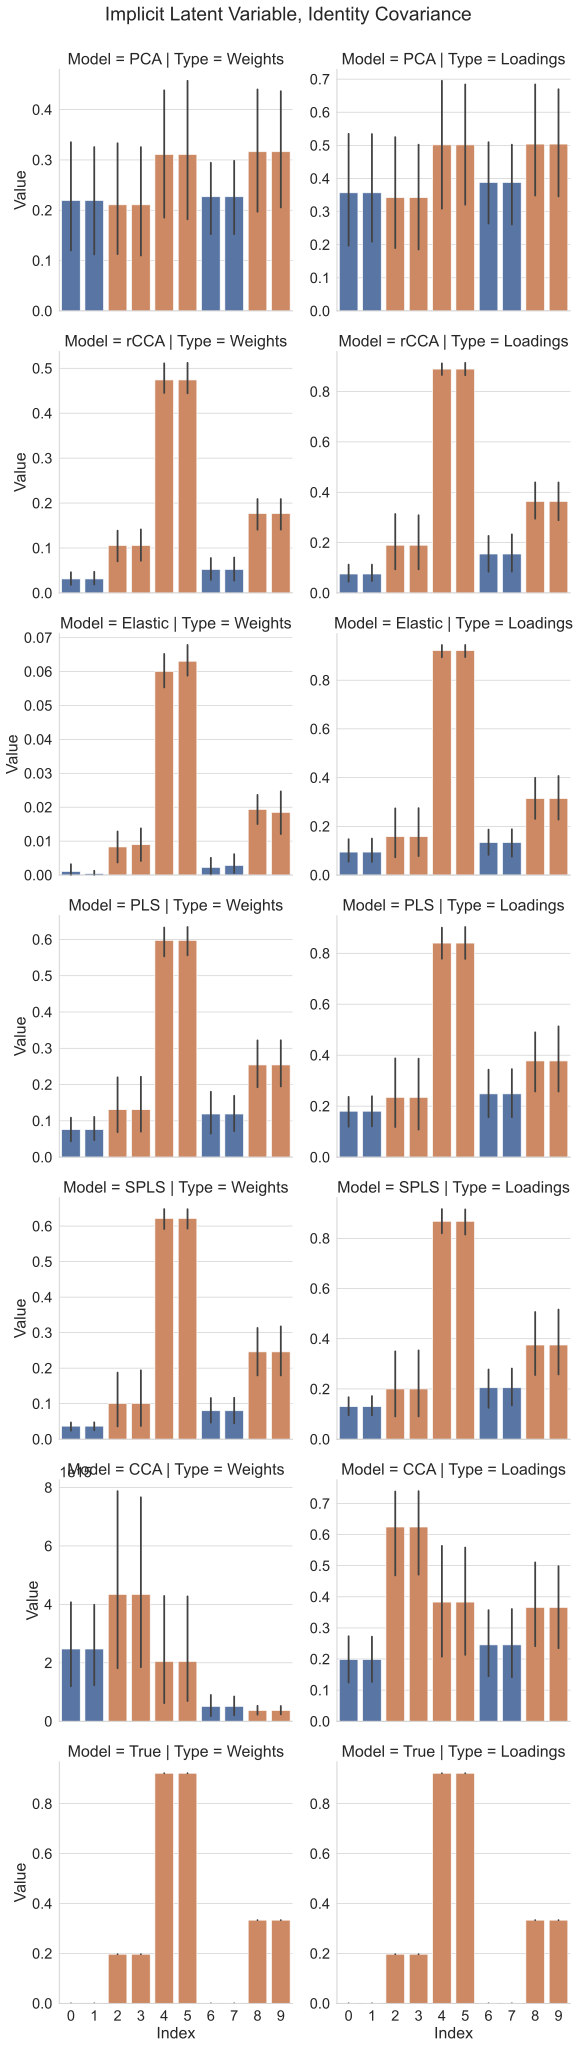
\includegraphics[width=\linewidth]{figures/simulated/low/Combined_Weights_Loadings_with_Error_Bars_Identity_Covariance_implicit}
        \caption{Identity Covariance Matrices}
    \end{subfigure}
    \begin{subfigure}{0.49\linewidth}
        \centering
        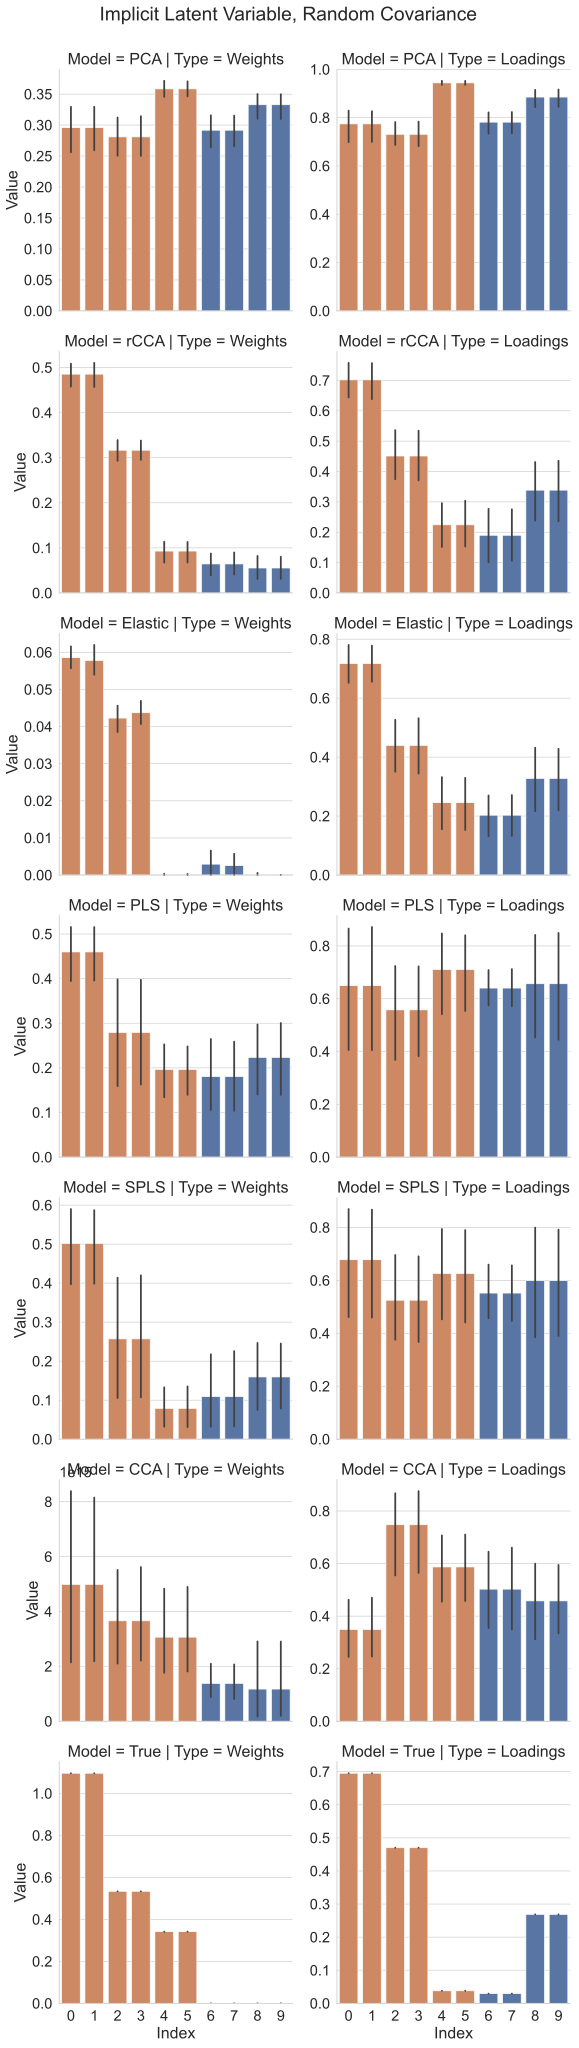
\includegraphics[width=\linewidth]{figures/simulated/low/Combined_Weights_Loadings_with_Error_Bars_Random_Covariance_implicit}
        \caption{Random Covariance Matrices}
    \end{subfigure}
    \caption{\textbf{Implicit Latent Variable:} Weights and Loadings. Blue signifies true zero weights and loadings, while Orange indicates estimated true non-zero weights and loadings.}\label{fig:implicit-latent-variable-weights-loadings}
\end{figure}

\paragraph{Recovery of Latent Variables}

Unregularized \acrshort{cca} and Ridge \acrshort{cca} are comparable to Elastic Net regularization but slightly worse in both scenarios (Figure \ref{fig:implicit-latent-variable-scores})

\begin{figure}
    \centering
    \begin{subfigure}{0.49\linewidth}
        \centering
        \includegraphics[width=\linewidth]{figures/simulated/low/Train_Test_Scores_Identity_Covariance_implicit}
        \caption{Identity Covariance Matrices}
    \end{subfigure}
    \begin{subfigure}{0.49\linewidth}
        \centering
        \includegraphics[width=\linewidth]{figures/simulated/low/Train_Test_Scores_Random_Covariance_implicit}
        \caption{Random Covariance Matrices}
    \end{subfigure}
    \caption{\textbf{Implicit Latent Variable:} Test Scores.}\label{fig:implicit-latent-variable-scores}
\end{figure}

\subsubsection{Explicit Latent Variables (Sparse Weights)}

\paragraph{Recovery of Weights and Loadings} A striking observation, though theoretically consistent, from Figure~\ref{fig:explicit-latent-variable-weights-loadings}a is that PCA almost perfectly recovers the true \gls{weights} and loadings for the \acrshort{gfa} model with identity noise covariance.
Admittedly, we have chosen a reasonably high signal-to-noise ratio for this experiment, but this nonetheless demonstrates that PCA can be a useful baseline for multiview data under an isotropic latent variable noise model.
Figure~\ref{fig:explicit-latent-variable-weights-loadings}b indicates that with anisotropic noise covariance, PCA no longer captures the true loadings.
There is no strong evidence that \acrshort{spls} or Elastic Net regularization outperform \acrshort{pls} or \acrshort{rcca}, respectively, in this setting.
This is unsurprising because the true \gls{weights} are not sparse, and so the additional sparsity constraints do not help.
However, this does illustrate that priors on \gls{weights} do not translate well to priors on loadings.

\begin{figure}
    \centering
    \begin{subfigure}{0.49\linewidth}
        \centering
        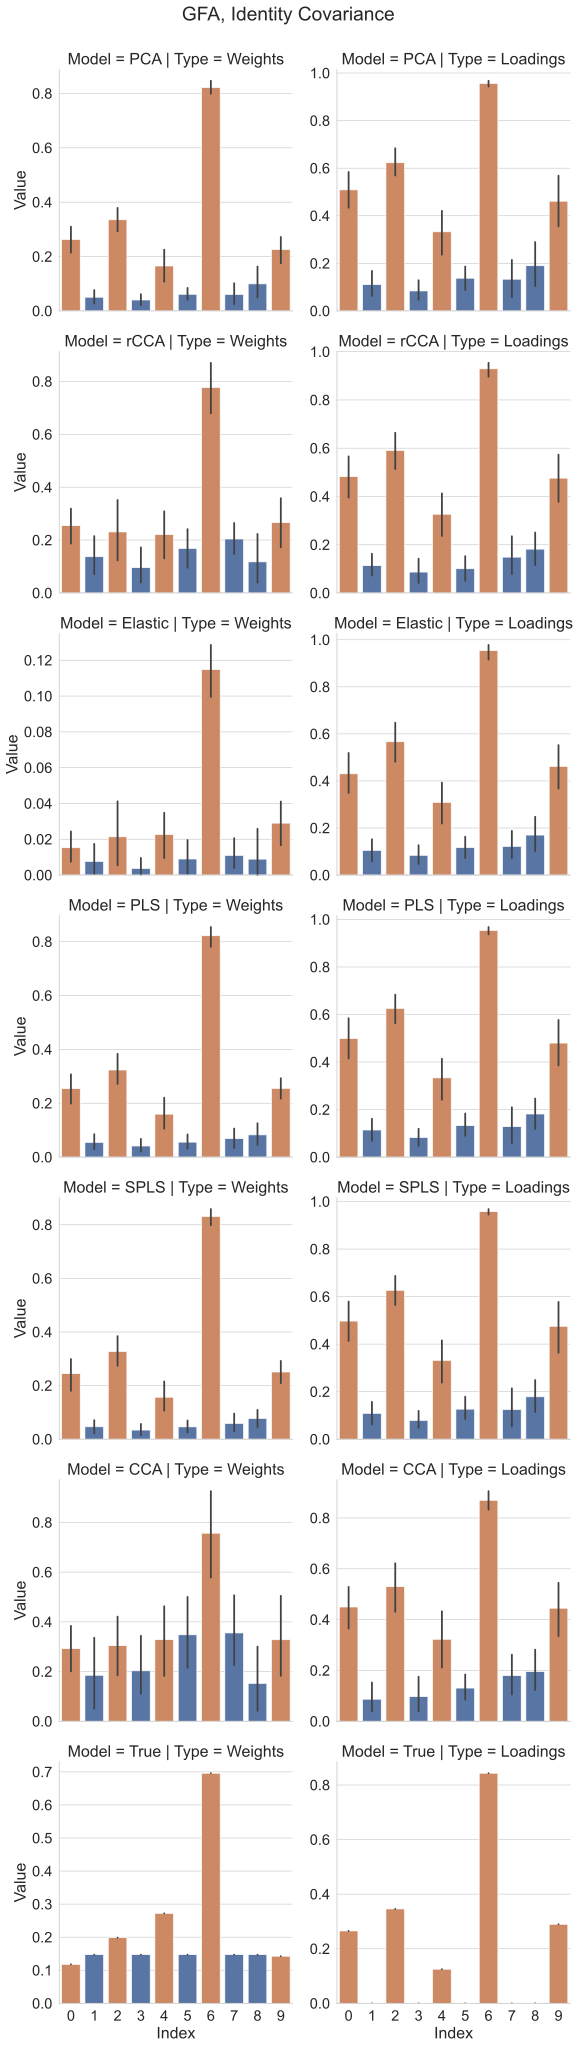
\includegraphics[width=\linewidth]{figures/simulated/low/Combined_Weights_Loadings_with_Error_Bars_Identity_Covariance_explicit}
        \caption{\acrshort{gfa} (Identity Noise)}
    \end{subfigure}
    \begin{subfigure}{0.49\linewidth}
        \centering
        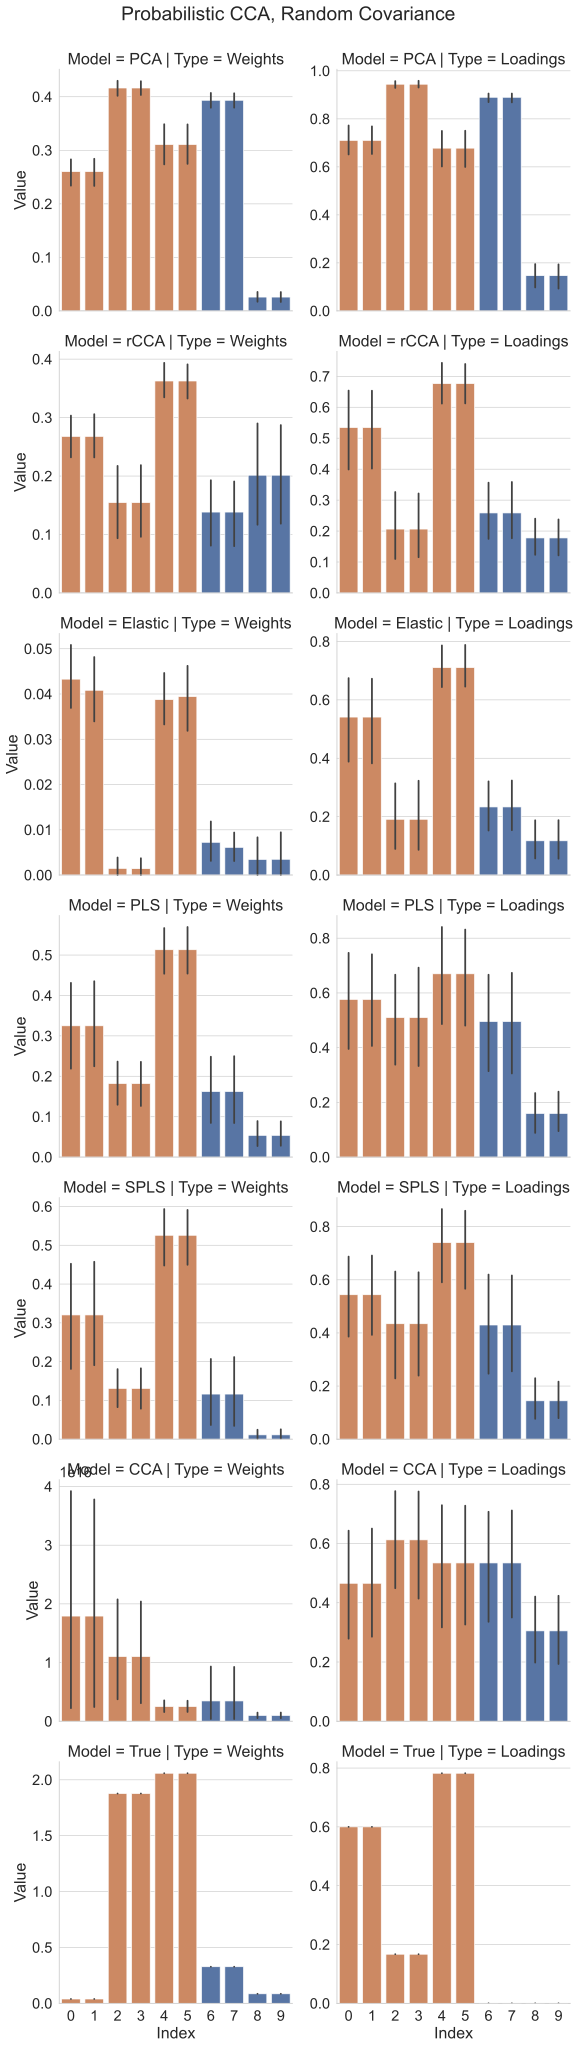
\includegraphics[width=\linewidth]{figures/simulated/low/Combined_Weights_Loadings_with_Error_Bars_Random_Covariance_explicit}
        \caption{Probabilistic \acrshort{cca} (Random Noise)}
    \end{subfigure}
    \caption{\textbf{Explicit Latent Variable:} Weights and Loadings. Blue signifies true zero weights and loadings, while Orange indicates estimated true non-zero weights and loadings.}\label{fig:explicit-latent-variable-weights-loadings}
\end{figure}

\paragraph{Recovery of Latent Variables}

Indeed, in the identity noise covariance scenario, all the models perform similarly (Figure~\ref{fig:explicit-latent-variable-scores}a) with the exception of \acrshort{cca} which appears to be unstable in this setting (Figure~\ref{fig:explicit-latent-variable-weights-loadings}a).
In the random noise covariance scenario, PCA performs poorly, and \acrshort{cca} now performs well (Figure~\ref{fig:explicit-latent-variable-scores}b).

\begin{figure}
    \centering
    \begin{subfigure}{0.49\linewidth}
        \centering
        \includegraphics[width=\linewidth]{figures/simulated/low/Train_Test_Scores_Identity_Covariance_explicit}
        \caption{\acrshort{gfa}}
    \end{subfigure}
    \begin{subfigure}{0.49\linewidth}
        \centering
        \includegraphics[width=\linewidth]{figures/simulated/low/Train_Test_Scores_Random_Covariance_explicit}
        \caption{Probabilistic \acrshort{cca}}
    \end{subfigure}
    \caption{\textbf{Explicit Latent Variable:} Test Scores.}\label{fig:explicit-latent-variable-scores}
\end{figure}

\subsubsection{Measuring the Identitiness of the Covariance Matrices}
The theory we developed in section~\ref{sec:generative-perspectives} suggests that the identitiness of the covariance matrices is crucial for understanding how imposing sparsity on the \gls{weights} imposes a prior belief in sparsity on the more biologically interesting loadings.
We can measure the identitiness of the covariance matrices by looking at the eigenvalues of the covariance matrices.
If the eigenvalues of the sample covariance matrix are all close to 1, then the sample covariance matrix is close to identity.
Departures from 1 indicate that the sample covariance matrix is not close to identity and imply multicollinearity in the data.

In the simulated data, we can see that the data generation models with identity noise covariance matrices, have eigenvalues closer to one than (Figure~\ref{fig:covariance-eigenvalues-simulated-low}).
On the other hand, these plots (shown for 10 random samples) show that all of the sample covariance matrices depart from the ideal case, \textit{even when the true covariance matrices are identity}.

\begin{figure}
    \centering
    \includegraphics[width=0.8\linewidth]{figures/covariance/simulated_covariance_eigenvalues_low}
    \caption{Eigenvalues of the covariance matrices for the simulated datasets.}\label{fig:covariance-eigenvalues-simulated-low}
\end{figure}


\subsection{Varying the Signal-to-Noise Ratio}

In Figures \ref{fig:snr-scores-identity} and \ref{fig:snr-scores-random} we plot the test correlation (score) varying the signal-to-noise ratio and the number of features.
Figure 

\begin{figure}
    \centering
    \includegraphics[width=\linewidth]{figures/simulated/snr/snr_vs_scores_facet_identity}
    \caption{Identity Covariance Matrices}\label{fig:snr-scores-identity}
\end{figure}

\begin{figure}
    \centering
    \includegraphics[width=\linewidth]{figures/simulated/snr/snr_vs_scores_facet_random}
    \caption{Random Covariance Matrices}\label{fig:snr-scores-random}
\end{figure}

\section{Revisiting Brain-Behaviour Results}

In this section, we revisit the results from the brain-behaviour experiments in Chapter \ref{chap:als} by comparing the weights and \gls{loadings} of the \acrshort{hcp} and \acrshort{adni} datasets.

\subsection{Identitiness of Covariance Matrices}
In this section, we consider the identitiness of the covariance matrices for the \acrshort{hcp} and \acrshort{adni} datasets.
Figure \ref{fig:covariance-eigenvalues-real} shows the eigenvalues of the covariance matrices for the \acrshort{hcp} and \acrshort{adni} datasets while Figure \ref{fig:covariance-matrices-real} shows the covariance matrices themselves (with the \acrshort{adni} brain covariance matrix left out due to its size).
From Figure \ref{fig:covariance-eigenvalues-real}, we can see that the eigenvalues of the covariance matrices for the \acrshort{adni} data are much closer to the ideal for identity covariance than for the \acrshort{hcp} data.
\begin{figure}
    \centering
    \includegraphics[width=0.8\linewidth]{figures/covariance/hcp_adni_covariance_eigenvalues}
    \caption{Eigenvalues of the covariance matrices for the \acrshort{hcp} and \acrshort{adni} datasets.}\label{fig:covariance-eigenvalues-real}
\end{figure}

From Figure \ref{fig:covariance-matrices-real}, we can see the block structure of the covariance matrices.

\begin{figure}
    \centering
    \begin{subfigure}{0.66\linewidth}
        \centering
        \includegraphics[width=\linewidth]{figures/covariance/hcp_covariance}
        \caption{\acrshort{hcp}}
    \end{subfigure}
%
    \begin{subfigure}{0.33\linewidth}
        \centering
        \includegraphics[width=\linewidth]{figures/covariance/adni_covariance}
        \caption{\acrshort{adni}}
    \end{subfigure}
    \caption{Covariance matrices for the \acrshort{hcp} and \acrshort{adni} datasets.}
    \label{fig:covariance-matrices-real}
\end{figure}

\subsection{Loading Similarity}

`\begin{figure}
     \centering
     \includegraphics[width=0.8\linewidth]{figures/hcp/brain and behaviour loadings correlation}
     \caption{\textbf{HCP:} Correlation between the brain and behaviour \gls{representations} for each model.}\label{fig:brain-behaviour-scores-sim}
\end{figure}

\subsection{Comparing Behaviour Weights and Loadings}

\subsubsection{Human Connectome Project (\acrshort{hcp}) Data}

\begin{figure}
    \centering
    \includegraphics[width=0.8\linewidth]{figures/hcp/PCA behaviour weights and loadings}
    \includegraphics[width=0.8\linewidth]{figures/hcp/RCCA behaviour weights and loadings}
    \includegraphics[width=0.8\linewidth]{figures/hcp/ElasticNet behaviour weights and loadings}
    \includegraphics[width=0.8\linewidth]{figures/hcp/PLS behaviour weights and loadings}
    \includegraphics[width=0.8\linewidth]{figures/hcp/SPLS behaviour weights and loadings}
    \caption{Top 8 positive and negative non-imaging \gls{loadings} for each model}
\end{figure}

\subsubsection{Alzheimer's Disease Neuroimaging Initiative (\acrshort{adni}) Data}

\begin{figure}
    \centering
    \includegraphics[width=0.8\linewidth]{figures/adni/PCA behaviour weights and loadings}
    \includegraphics[width=0.8\linewidth]{figures/adni/RCCA behaviour weights and loadings}
    \includegraphics[width=0.8\linewidth]{figures/adni/ElasticNet behaviour weights and loadings}
    \includegraphics[width=0.8\linewidth]{figures/adni/PLS behaviour weights and loadings}
    \includegraphics[width=0.8\linewidth]{figures/adni/SPLS behaviour weights and loadings}
    \caption{Bar plots of the behaviour \gls{weights} and \gls{loadings} for each model.}
\end{figure}

\section{Discussion}

In this section, we discuss the implications of our findings.

\paragraph{Interpreting the Forward and Backward Models of \acrshort{cca}:} Consistent with \cite{haufe2014interpretation}, we have shown that assumptions imposed on the \gls{weights} of a model do not in general transfer to the loadings.
This is because the \gls{weights} and \gls{loadings} are only equivalent when the covariance matrices are identity.
We have gone a step further than \cite{haufe2014interpretation} by showing that the identitiness of the covariance matrices is crucial for understanding how imposing sparsity on the \gls{weights} imposes a prior belief in sparsity on the more biologically interesting loadings.

\paragraph{Identitiness of real covariance matrices:} Between the \acrshort{hcp} and \acrshort{adni} datasets, only the \acrshort{adni} data had eigenvalue spectra that were reasonably close to those of an identity matrix.
This suggests that the only dataset and view where we can expect sparsity on the \gls{weights} to imply sparsity on the \gls{loadings} is the \acrshort{adni} data.
This is consistent with the results we have seen in the previous section, that sparsity improves performance in the \acrshort{adni} data but not in the \acrshort{hcp} data.
Furthermore, the \gls{loadings} and \gls{weights} are much more similar to each other in the \acrshort{adni} data than in the \acrshort{hcp} data, supporting the idea that the \acrshort{adni} \gls{weights} are themselves somewhat interpretable as estimates of the biologically relevant loadings.
Finally, in the well understood Alzheimer's disease data, we know that the identified \gls{weights} (and loadings) are consistent with the known biology of the disease.

\paragraph{Sample versus Population Setting:} The results from the simulated data illustrate the disparities that can arise between population and sample settings.
Although \acrshort{pls}, \acrshort{rcca}, and \acrshort{cca} are equivalent under isotropic noise in a population framework, experiments showed that their performance can vary substantially in a sample setting.
In particular, this manifested as \acrshort{pls} underperforming \acrshort{rcca} and \acrshort{cca} under isotropic noise \textit{even though this is exactly the scenario where covariance identity holds and covariance thus equals correlation}.
This is because the sample covariance matrix is not the same as the population covariance matrix and \acrshort{pls} is sensitive to even small differences in the principal components of the sample covariance matrix.
Furthermore, in limited sample sizes, our estimations of the covariance matrices are not accurate, and so the identitiness of the covariance matrices is not guaranteed.
This generally resulted in poor estimation of \gls{loadings} from model \gls{weights} \textit{even when the \gls{weights} themselves were estimated almost perfectly}.
Therefore, it's crucial for researchers to recognize these nuances and adopt appropriate measures when extrapolating results, especially in brain-behaviour studies where typically only one sample is available and often limited in size.


\paragraph{Can We Construct a Regularization Functional that Imposes Sparsity on the Loadings?}
Finally, given our observations, a natural question to ask is whether we can construct a regularization functional that imposes sparsity on the \gls{loadings} (instead of the weights).
The answer is yes, but it is not straightforward and in the small sample setting, it is not clear that it is a good idea.
The principle would be much the same as the Lasso, but we would need to use the sample covariance matrix to define the norm:

\begin{align}
    P(W)=\|W\|_1 \\
    P(L)=\|\hat{\Sigma}U\|_1
\end{align}

Which imposes an L1 penalty on the \gls{loadings} via an L1 penalty on the \gls{weights} multiplied by the sample covariance matrix.
We could in principle apply the soft-thresholding operator to the estimated loadings.
However we would need to be careful to ensure that the sample covariance matrix is invertible in order to get back to the weights.
This is of course not guaranteed in the small sample setting.

\section{Conclusion}

In this chapter, we have shown that the \gls{loadings} are of critical importance for the interpretation of \acrshort{cca} models.
We have shown that the \gls{loadings} are invariant to columnwise transformations of the data matrix, while the \gls{weights} are not.
Through a series of experiments, we have demonstrated that the \gls{loadings} are more stable than the \gls{weights} across datasets and samples.
We have also shown that regularisation of the \gls{weights} does not imply regularisation of the \gls{loadings}.
Finally, we have shown that the identitiness of the covariance matrices is crucial for understanding whether imposing sparsity on the \gls{weights} imposes a prior belief in sparsity on loadings.
We revisited the results of chapter~\ref{chap:frals} and showed that our interpretations would be different if we used \gls{loadings} instead of \gls{weights}.